


\chapter{Input Output}



\section{LED program}

Our $\mathrm{1}^\mathrm{st}$ program to HLS will be driving some LED on.

Now we will proceede in each section for a specific step from programming until bitstream file used in the fpga.\\

\todo{LED Controller} \uti{LED Controller:}

\begin{itemize}

\item \textit{To re-write the statment properly with some images}

\item \textit{To illustrate again the concept of:}

	\begin{itemize}
	\item \textit{interfaces}
	
	\item \textit{Port and pins conncetion}
	
	\item \textit{Role of pragma directive}
	\end{itemize}

\end{itemize}


\subsection{Resource for the Vitis IDE}

Refer to \url{https://docs.amd.com/r/en-US/ug1399-vitis-hls/Building-and-Running-an-HLS-Component} to see:

\begin{itemize}

\item Vitis IDE structure

\item Different Steps when building and desiging an HLS component

\end{itemize}

\todo{Vitis IDE} \uti{Vitis IDE:}

\begin{itemize}

\item \textit{To illustrate and make some introduction about the content of the url}

\item \textit{Mainly about:}

	\begin{itemize}
	
	\item \textit{The steps and the process}	
	
	\item \textit{The options in Vitis IDE with some images}
		
	\end{itemize}


\end{itemize}


\subsection{Generating IP Package}

After running successfully the \verb|C| simulation step, we need to generate an IP pacakge. This package can be used in \verb|Vivado| software so we can generate the bitstream file which will be used to program the FPGA.\\

\underline{Generating the IP Pacakge:} under the flow navigator, run the \verb|Package| command, and we should specify the 


\subsection{Vivado}

Now we are ready to generate the bitstream file. For that, open \verb|Vivado|, and create a project.\\

Then \verb|Create IP block diagram|.

Under \verb|Settings|, search for the \verb|IP| workspace, and \verb|Vivado| will search for any \verb|IP| in the selected workspace.



We can search for our \verb|IP| name (\verb|basic_output|), then using the search bar select the \verb|IP| name we want, and the block will be imported to \verb|Vivado| as shown in \autoref{fig:input_output:ip_block}.

\begin{figure}[h]
\centering
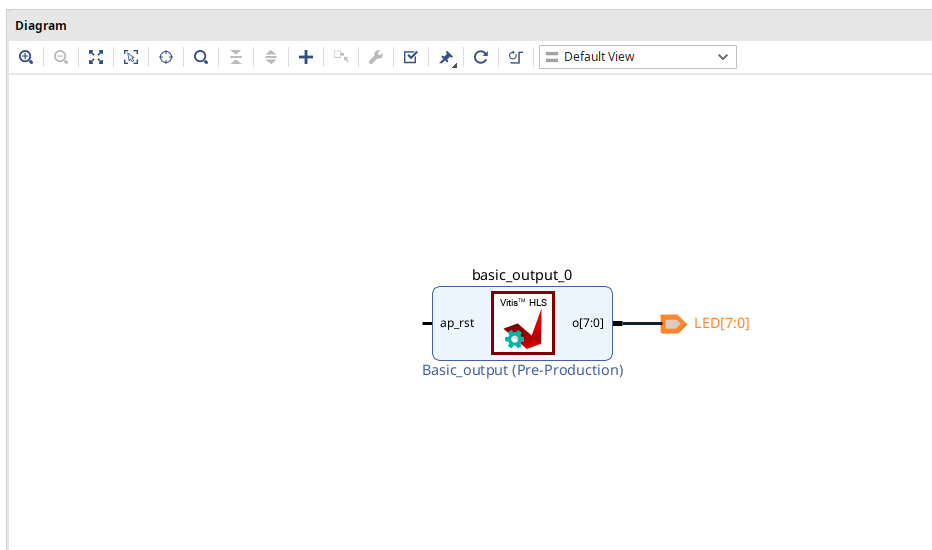
\includegraphics[scale=0.5,frame]{Figures/input_output/ip_block}
\caption{IP Block for LED controller}
\label{fig:input_output:ip_block}
\end{figure}


\underline{Port to FPGA Pins: Constrains}\\

Now to make connections form the port of the \verb|IP| to the FPGA pins, we need to some constraints. To add these constraints, go \verb|Sources|, right click on \verb|Constraints| folder and select \verb|Add Sources|.\\

After that we select \verb|Create Constraint| option, and then choose a file name.\\

We copy paste the constraint file forom \verb|digilent| gihtub for basys3 board (\url{https://github.com/Digilent/Basys3/tree/master}). under \verb|Resources| folder.\\

Finally we uncomment the $\mathrm{1}^\mathrm{st}$ 8 LED in the LED sections.







